\par Para elaboração do sistema \emph{PID} que tenha a performance desejada, mantendo o equipamento \emph{LASER} nos parâmetros de operação desejados usarei as técnicas de Engenharia de Controle para modelar o sistema através das equações de transferência do sistema.\\

Para elaborarmos a Equação de Transferência para o sistema temos que seguir o seguinte diagrama de blocos genérico:

\begin{figure}[H]
		\centering
		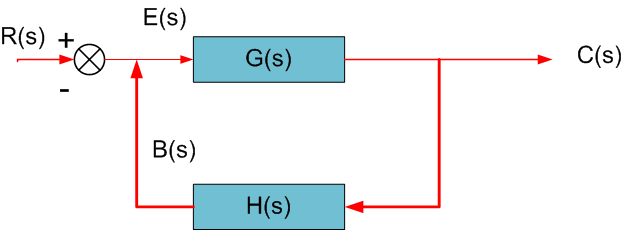
\includegraphics[width=0.7\linewidth]{./ima/DiagramaDeBlocos02Ftranferencia.png}
		%\caption{}
		\label{fig:FuncTransf}
		\caption{Diagrama de Bloco Func. Transferência}
	\end{figure}
	
Assim para esse diagrama de blocos, podemos formular a seguinte equação:

\[\frac{C(s)}{R(S)}= \frac{G(s)}{1+G(s)H(s)}\]

Ainda referente ao cronograma do processo, após termos identificado as questões 1 e 2, do organograma da figura 1 \label{fluxo1}, e conhecendo os dados genéricos de uma função de transferência, passamos a tratar de escrever as especificações das variáveis desta equação de transferência ( item 3 da mesma figura ).

É necessário que se tenha  bem estudada e planejada tal função, para  obter um sistema de alta performance em sua aplicação. Dispondo deste conhecimento, o mesmo sirva para novas implementações e garante que ao se necessitar de alterações tenha-se todo o histórico e o tratamento analítico do processo de projeto. 

Tecnicamente, que vem a ser a importância maior neste trabalho o sistema tendo sua \emph{Função de Transferência} garante que o sistema atenda as necessidades do projeto com a máxima precisão, pois no decorrer do projeto, caso haja necessidade, esta Função pode ir sendo alterada e melhorada a cada avanço.
